\documentclass{standalone}
\usepackage{tikz,amsmath}
\tikzset{block/.style = {draw, fill=white, very thick, rectangle, minimum height=1cm, minimum width=2cm},}
\tikzset{sum/.style= {draw, fill=white, very thick, circle, node distance=1cm},}
\begin{document}
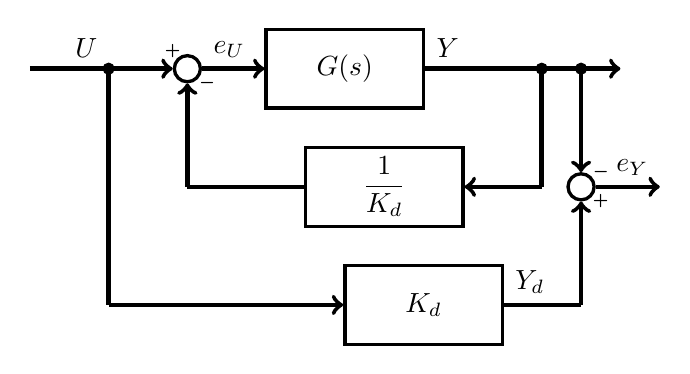
\begin{tikzpicture}[scale=2]
    \node[sum](sum)at(-1,0){};
    \draw[->,ultra thick](-1.5,0)--(sum.180)node[above]{$\scriptscriptstyle\boldsymbol{+}$};
    \draw[-,ultra thick](-2,0)--(-1.5,0)node[above left]{$U$};
    \filldraw[black](-1.5,0)circle(1pt);
    %\node[triangle, right of=sum, node distance=2cm](c){$K_c$};

    %\draw[->,ultra thick](sum.0)--(c.180);
    \filldraw[black](1.25,0)circle(1pt);
    \filldraw[black](1.5,0)circle(1pt);
    \draw[-,ultra thick](1.25,0)--(1.5,0);
    \draw[->,ultra thick](1.5,0)--(1.75,0);

    %\draw[->,ultra thick](2.5,0)--(3,0)node[above left]{$Y$};
    %\draw[-,ultra thick](2.5,-0.75)--(2.5,0);

    \node[block]at(0.25,-0.75)(h){$\displaystyle\frac{1}{K_d}$};
    \node[block, right of=sum, node distance=2cm](p){$G(s)$};
    \draw[->,ultra thick](sum.0)node[above right]{$e_U$}--(p.180);
    \draw[-,ultra thick](p.0)node[above right]{$Y$}--(1.25,0);
    %\draw[->,ultra thick](c.0)--(p.180);

    \draw[-,ultra thick](1.25,0)--(1.25,-0.75);
    \draw[->,ultra thick](1.25,-0.75)--(h.0);
    \draw[-,ultra thick](h.180)--(-1,-0.75);
    %\draw[-,ultra thick](2.5,-0.75)--(-1,-0.75);
    \draw[->,ultra thick](-1,-0.75)--(sum.270)node[right]{$\scriptscriptstyle\boldsymbol{-}$};

    \node[sum](sum2)at(1.5,-0.75){};
    \draw[->,ultra thick](1.5,0)--(sum2.90)node[right]{$\scriptscriptstyle\boldsymbol{-}$};
    \node[block](k)at(0.5,-1.5){$K_d$};
    \draw[-,ultra thick](k.0)node[above right]{$Y_d$}--(1.5,-1.5);
    \draw[->,ultra thick](1.5,-1.5)--(sum2.270)node[right]{$\scriptscriptstyle\boldsymbol{+}$};

    \draw[-,ultra thick](-1.5,0)--(-1.5,-1.5);
    \draw[->,ultra thick](-1.5,-1.5)--(k.180);

    \draw[->,ultra thick](sum2.0)--(2,-0.75)node[above left]{$e_Y$};
\end{tikzpicture}
\end{document}